\section{梁のモーダル解析}
この例では、単純支持された長方形の梁を、固有振動数の観点から解析します。その寸法は:
\begin{itemize}
\item 断面:正方形40 mm
\item 長さ:1000mm
\end{itemize}
\begin{enumerate}
\item
  {[}mm, ton, s, °C{]}単位の新規ファイルを作成し、ステップ形式のジオメトリをPrePoMaxにインポートします。
  次に、パーツをメッシュ分割します。
  ここでは、最大要素サイズとして10mmを選択し、その他の設定は変更しませんでした(図\ref{fig:06-01})。
	\begin{figure}[H]
	\centering
	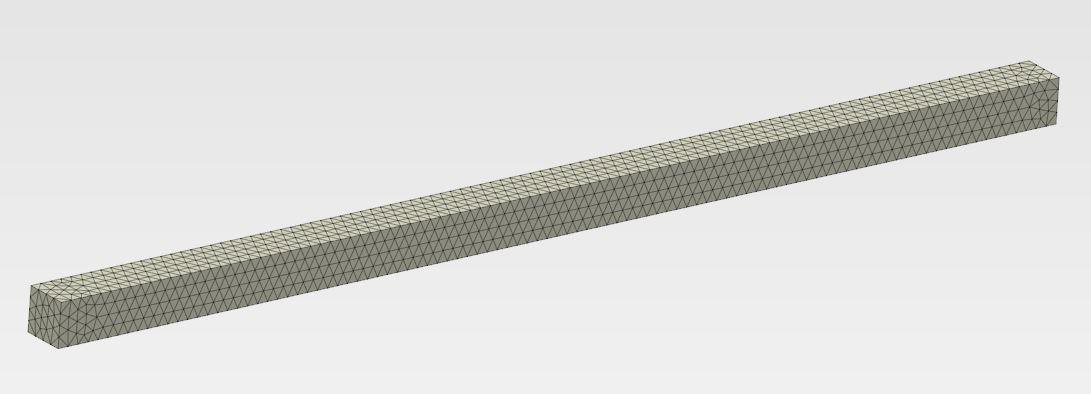
\includegraphics[width=143mm]{fig/06-01.png}
	\caption{梁 - メッシュ}
	\label{fig:06-01}
	\end{figure}
\item
  新しい材料を定義し、弾性挙動を加え、ヤング率を210000MPa、ポアソン比を0.3と指定します。
  また、Density(密度)を追加し、7.85e-9tont/mm3の値を指定します。
  先に作成した材料を参照して新しいソリッドセクションを作成し、そのセクションがこのパーツに割り当てられるように梁を選択します。
\item
  デフォルトの設定で周波数ステップを作成します(10個の固有振動数の抽出)。変位/回転境界条件を一方の端の断面の下部エッジに適用します。
  自由度U1、U2、U3を固定します。
  反対側の断面の下部エッジに適用される別の変位/回転境界条件を作成します。
  先ほどと同様に自由度を固定しますが、ローラー支持をシミュレートするために、1つの移動(ビームの軸方向の移動)を残します(図\ref{fig:06-02})。
	\begin{figure}[H]
	\centering
	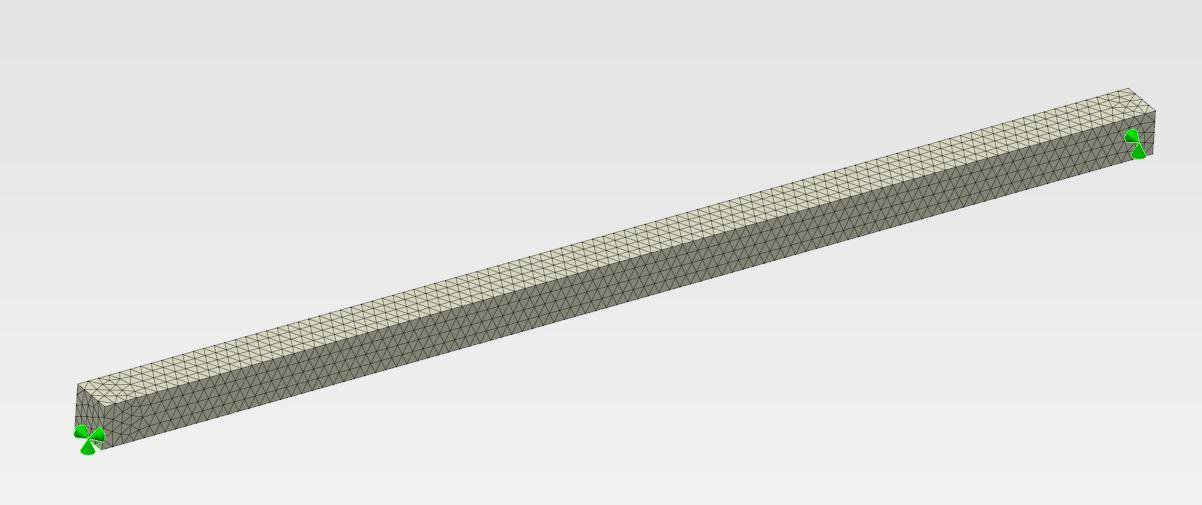
\includegraphics[width=145mm]{fig/06-02.png}
	\caption{梁 - 境界条件}
	\label{fig:06-02}
	\end{figure}
\item
  解析を実行し、解析が完了したら結果を開きます。
  固有振動数とモード形状を調べます。
  モード形状を切り替えるには、Previous/Nextの増分ボタン、またはショートカットツールバーのドロップダウンリストを使用します。
  固有振動数の解析値を以下に示します(表\ref{tab:06-01})。
\end{enumerate}
\begin{table}[H]
\centering
\caption{梁 - 理論固有振動数}
\label{tab:06-01}
\begin{tabular}{|c|c|}
\hline
No. & 固有振動数    \\
    & {[}Hz{]} \\ \hline
1   & 93.82    \\ \hline
2   & 375.46   \\ \hline
3   & 844.07   \\ \hline
4   & 1501.83  \\ \hline
5   & 2347.80  \\ \hline
\end{tabular}
\end{table}
一方、解析で得られた値は次の表(表\ref{tab:06-02})のとおりです。
\begin{table}[H]
\centering
\caption{解析による梁の固有振動数}
\label{tab:06-02}
\begin{tabular}{|c|c|}
\hline
No. & 固有振動数    \\
    & {[}Hz{]} \\ \hline
1 & 93.39\\ \hline
2 & 121.28\\ \hline
3 & 339.68\\ \hline
4 & 413.17\\ \hline
5 & 785.76\\ \hline
6 & 850.47\\ \hline
7 & 1066.7\\ \hline
8 & 1223.69\\ \hline
9 & 1478.86\\ \hline
10 & 1609.22\\ \hline
\end{tabular}
\end{table}
解析計算は簡略化されており(1つの平面内の変形のみを考慮している)、モーダル解析で得られたすべての固有振動数を予測することはできません。これが、この場合の結果の違いの主な理由の1つです。
\vskip\baselineskip
下の画像では、高次モードの形状の1つ(\#9)を見ることができます(図\ref{fig:06-03})。
\begin{figure}[H]
\centering
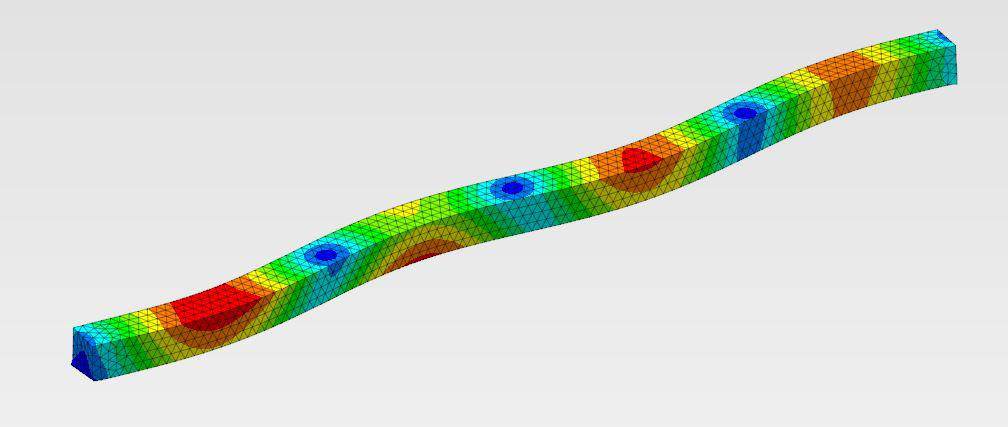
\includegraphics[width=133mm]{fig/06-03.png}
\caption{梁 - モード形状 \#9}
\label{fig:06-03}
\end{figure}